\documentclass{article}
\usepackage{ctex}
\usepackage{geometry}
\geometry{top = 2cm, left = 1cm, right = 1cm, bottom = 2cm}
\usepackage{amsmath,amssymb,amsthm,amsfonts}
\usepackage{abstract}
\usepackage{siunitx}
\usepackage{graphicx}
\usepackage{booktabs}
\usepackage{appendix}
\usepackage{hyperref}
\usepackage{lscape}
\usepackage{multirow}

\renewcommand{\appendixpagename}{附录}


\title{利用逆矩阵法解$\gamma$谱}
\author{钱思天 2001112187}
\begin{document}
    \maketitle
    \begin{abstract}
        本实验通过逆矩阵法,根据对已知$^{60}\text{Co},^{137}\text{Cs}$源的测量,对未知混合源中的各核素活度进行了测量,并进行了误差分析。
        \newline
        \newline
        {\emph{ 关键词:\ 逆矩阵、$\gamma$射线谱、能量刻度 }\rm}

    \end{abstract}

    \section{实验介绍}
    \subsection{实验原理}
    用逆矩阵法解析复杂γ能谱时,对各种成分放射性含量比较相近的样品,解谱误差可达 2\%左右。对弱成分误差显著增大。

    利用逆矩阵法解谱,要能得到准确的结果,必须满足下列条 件:(1).混合样品中核素都是已知的。(2).测量标准谱和混合样品谱 时,谱仪的测量条件一致,仪器要求稳定。(3).各单一核素放射性线 性叠加情况下,探测系统的脉冲幅度不随计数率改变。(4).混合样品 中各核素具有各自的γ能谱,并能够选出表征各自能量的特征峰。
现混合样品由多种核素组成,这些核素含有 137Cs, 60Co。在混合样品的$\gamma$射线谱中,对这两种核素选择一个能够表征各自能量的特征峰。又能区别于其他核素的全能峰,成为该核素的 特征全能峰。在这个全能峰上选择一个对应于最高计数处的道域称 为特征道域。测量每个核素标准谱时,不仅要测量它在本身的特征 道域中的计数,而且要测出它在其它特征道域中的计数,由此来确 定各种核素对每个道域计数的贡献,这个贡献用响应系数$a_{ij}$来表示,$a_{ij}$为谱仪$i$道对第$j$种核素的响应系数。定义为:
\begin{equation}
    a_{ij}=\frac{\text{第}j\text{种核素标准谱在第}i\text{道上的计数率}}{\text{第}j\text{核素标准样品的衰变率}}
\end{equation}
此响应系数取决于第$j$种成分各$\gamma$射线的相对强度和谱仪的测量条件。其意义是第$j$种核素的衰变率在$i$道域上引起的计数率。

    对混合样品,要测量在各个特征道域中引起的计数。如果第$j$道域上的计数率为$m_1,m_2$,各核素对任一道域上的计数都 有贡献。因此,混合样品在任意一道域中的计数率可以分解为各个 核素分别在该道域中引起的计数率之和。
    \begin{equation}
        \sum_{j = 1,2} a_{ij}x_{j} = m_i, i = 1,2 
    \end{equation}
    这样就得到一个由三个方程组成的联立方程组。此方程组可以用逆
    矩阵法求解。将方程组改写成矩阵形式
    \begin{equation}
        A\cdot X = M;A=\begin{pmatrix}
            a_{11}&a_{12}\\a_{21}&a_{22}
        \end{pmatrix};X=\begin{pmatrix}
                x_1\\x_2
            \end{pmatrix};M=\begin{pmatrix}
                m_1\\m_2
            \end{pmatrix}
    \end{equation}
    从而可得:\begin{equation}
        X = A^{-1}\cdot M
    \end{equation}

    因此,由实验测定$A$,求得$A^{-1}$。再把测得各特征道域上的计数率 $m_i$代入,即可算出该混合样品中各核素的活度$x_j$。

    被测样品在各特征道域上的计数和谱仪本底都会有统计涨落, 并通过逆矩阵计算相互传递。假如标准谱的测量精度足够高,使响 应系数的误差可以忽略。根据误差理论可以推算出第$j$成分含量$x_j$的标准误差$\sigma_{x_j}$为\footnote{推导见附录}
    \begin{equation}
        \begin{aligned}
            \sigma_{x_j} &= \frac{1}{\sqrt{t}}\sqrt{(\Delta\cdot X)_j+B_j}\\
            \Delta &= \{\sum_{j'}(A^{-1}_{ij'})^2A_{j'j}\} \\
            B_j &= 2\sum_{j'}(A^{-1}_{ji})^2b_{i} 
        \end{aligned}
    \end{equation}
    其中$b_i$为$i$道域的本底计数率。$t$为样品测量时间。
    \subsection{实验目的}
    \begin{enumerate}
        \item 了解逆矩阵法解析复杂$\gamma$谱的基本原理。
        \item 测量混合样品中各核素的未知活度。
    \end{enumerate}
    \section{实验器材与步骤}
    \subsection{实验器材}
    \begin{enumerate}
        \item FJ374 闪烁探头 1 个;
        \item BH1324多道分析器1台;
        \item 标准样品一套($^{60}\text{Co},^{137}\text{Cs}$);
        \item 混合样品一个;
    \end{enumerate}
    \subsection{实验步骤}
    \begin{enumerate}
        \item 检查仪器连接,预热 10 分钟。打开微机。
        \item 调整 NaI(Tl)$\gamma$谱仪参量工作电压推荐值 $650\si{V}$。
        \item 测量$^{137}\text{Cs}, ^{60}\text{Co}$标准样品的$\gamma$谱,测量时间 1200 秒,做出能量刻度曲线。用$^{137}\text{Cs}$全能峰($0.662\si{MeV}$)确定谱仪能 量分辨率。
        \item 分别测量混合样品(未知活度)能谱及本底谱。
        \item 合理选择特征道域(20~40 道)。列联立方程,自编程序用逆 矩阵法解方程,求出混合源中各组分现在的活度$x_j$,并计算误差
        $\sigma_{x_j}$。
    \end{enumerate}
    \section{实验数据}
    实验中测量得到的能谱图见附录。
    \subsection{能谱峰测量及刻度}
    实验中对已知源的刻度测量结果如表\ref{tab:Calibration}。
    \begin{table}[htbp]
        \centering
        \caption{实验中利用已知源的刻度结果\label{tab:Calibration}}
        \begin{tabular}{ccccc}
\toprule
          Element &  Peak Energy$[\si{KeV}]$ &  Channel &  Count &  Live time$[\si{s}]$ \\
\midrule
 \multirow{2}{*}{$^{60}\text{Co}$} &                   1332.5 &      815 &  16035 &     \multirow{2}{*}{1011} \\
              &                   1173.2 &      720 &  21507 &         \\
$^{137}\text{Cs}$ &                    661.7 &      403 &  53748 &     1100 \\
\bottomrule
\end{tabular}

    \end{table}

    刻度结果为\begin{equation}
        E = 1.6245 * \text{Ch} + 6.3869
    \end{equation}

    回归结果如图\ref{fig:Calibration}。
    \begin{figure}[htbp]
        \centering
        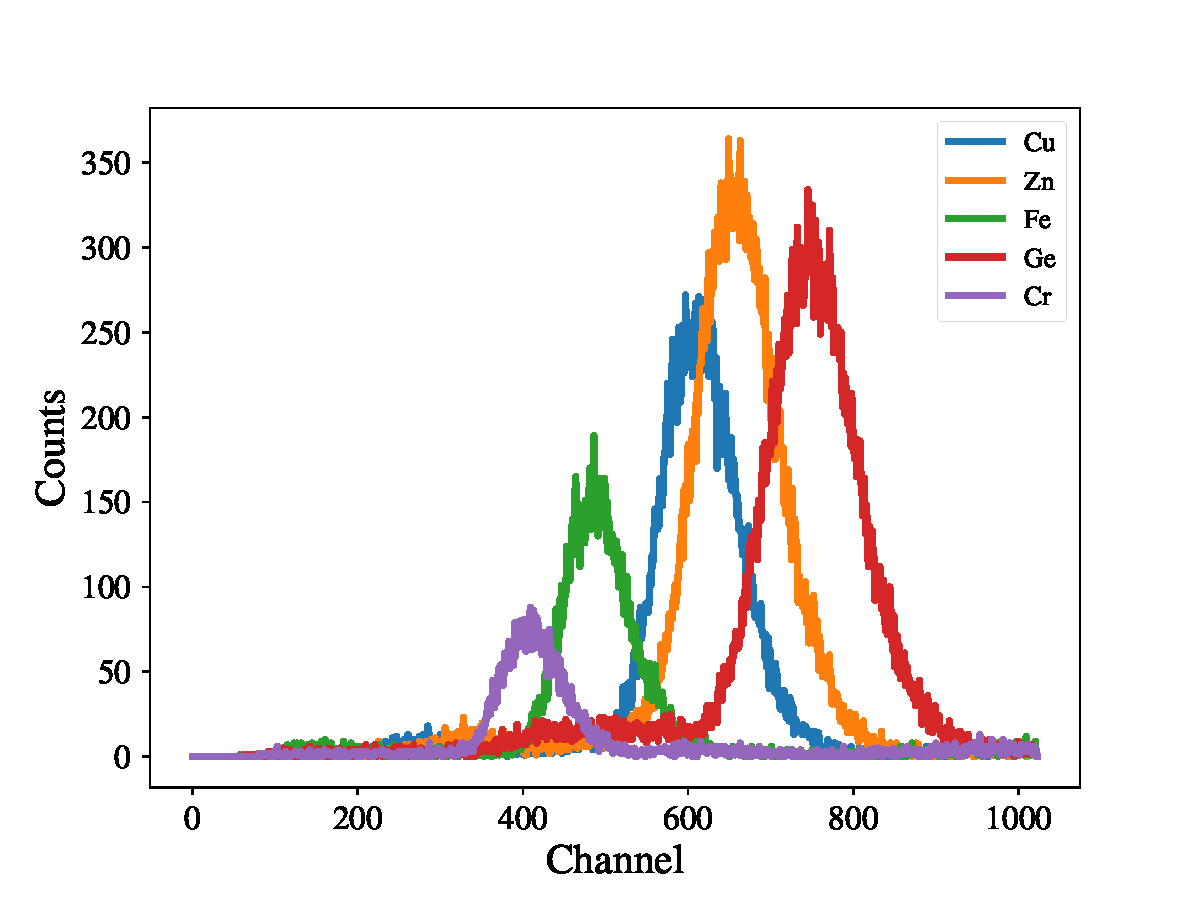
\includegraphics[width=0.7\textwidth]{../plots/Calibration.pdf}
        \caption{实验中利用已知源的刻度结果\label{fig:Calibration}}
    \end{figure}
    \subsection{能量分辨率}
    利用$^{137}\text{Cs}$源的全能峰,可以对实验装置的分辨率做出评价:
    \begin{enumerate}
        \item 峰位道址:403
        \item FWHM:36.7
        \item 能量分辨率:9.1\%
    \end{enumerate}
    \subsection{利用逆矩阵法解$\gamma$谱}
    首先利用半衰期与活度的关系\begin{equation}
        A = A_0\exp(-\frac{t}{T}\ln{2})
    \end{equation}
    
    计算实验当日的已知源活度如表\ref{tab:Source}
    \begin{table}[htbp]
        \centering
        \caption{实验当日的活度信息\label{tab:Source}}
        \input{SourceInfo.csv}
    \end{table}

    对于实验采用的$^{60}\text{Cs}$,$^{137}\text{Cs}$源,在其峰位左右对称选取30道,其峰的道址范围分别如表\ref{tab:Region}。
    \begin{table}[htbp]
        \centering
        \caption{道址的选取范围\label{tab:Region}}
        \begin{tabular}{llrrr}
\toprule
Label & Element &  Peak &  Left &  Right \\
\midrule
1     &      Co &   815 &   800 &    830 \\
2     &      Cs &   403 &   388 &    418 \\
\bottomrule
\end{tabular}

    \end{table}

    得到计数分别如表\ref{tab:Count}。
    \begin{table}[htbp]
        \centering
        \caption{各区域各样品计数\label{tab:Count}}
        \begin{tabular}{lrrr}
\toprule
{} &  R1 Count &   R2 Count &  Live Time/s \\
\midrule
Co      &  467669.0 &   335005.0 &       1011.0 \\
Cs      &     781.0 &  1456700.0 &       1110.0 \\
Unknown &  290688.0 &  1142768.0 &       1023.0 \\
BKG     &     132.0 &      665.0 &       1200.0 \\
\bottomrule
\end{tabular}

    \end{table}

    可以计算出
    \begin{equation}
        A = \begin{pmatrix}
            3.4922\times10^{-3}&1.4489\times10^{-5}\\
       2.4979\times10^{-3}&3.2020\times10^{-2}
        \end{pmatrix}
    \end{equation}
    故有
    \begin{equation}
        A^{-1} = \begin{pmatrix}
            286.4437  & -0.1296\\
  -22.3462  & 31.2403
        \end{pmatrix}
    \end{equation}
    根据\begin{equation}
        M = \begin{pmatrix}
            284.0425\\1116.5211
        \end{pmatrix}
    \end{equation}
    得到\begin{equation}
        X = \begin{pmatrix}
            81217\\28533
        \end{pmatrix}
    \end{equation}
    根据误差传递公式,得到:
    \begin{equation}
        \sigma_{X} = \begin{pmatrix}
            146\\
   33
        \end{pmatrix}
    \end{equation}
    得到最终结果
    \begin{equation}
        X+\sigma_{X} = \begin{pmatrix}
            81217 \pm 146\\
            28533\pm33
        \end{pmatrix}
    \end{equation}
\section{致谢}
    感谢许金艳老师的指导,也感谢张轩豪同学和蒋沛成同学一起进行实验。 
    \clearpage
    \appendix
    \appendixpage
    \section{思考题}
    \begin{enumerate}
        \item 主对角线上的数越高,探测效率约高。其余元素越低,探测
        效率越高。在实验中,因为要换源,几种源可能会相互影响,降低 探测效率。
        \item 利用逆矩阵法解谱,要能得到准确的结果,必须满足下列条
        件:(1).混合样品中核素都是已知的。(2).测量标准谱和混合样品谱 时,谱仪的测量条件一致,仪器要求稳定。(3).各单一核素放射性线 性叠加情况下,探测系统的脉冲幅度不随计数率改变。(4).混合样品 中各核素具有各自的γ能谱,并能够选出表征各自能量的特征峰。
        本次实验中混合源已知为$^{137}\text{Cs}$和$^{60}\text{Co}$的混合, 它们的全能峰都比较突出且不重叠。实验时高压和放大倍数不变,测 量时间也保持不变,在放置样品时尽量保持位置不变,因此满足了利 用逆矩阵方法解谱的条件。
        \item 以某一特征峰的峰址为中心,左右对称选择 20-40 道范围。道 域太窄,系统的统计涨落的影响比较大;道域太宽,低统计量的部分 会受到本底及康普顿平台的影响。
    \end{enumerate}
    \section{误差公式的推导}
    记$\tilde{M}$为总计数,则:
    \begin{equation}
        M = \tilde{M} - b
    \end{equation}
    那么,在忽略$A$的误差的情况下,有:
    \begin{equation}
        \begin{aligned}
            \sigma_{x_j}^2 &= \frac{1}{t}\sum_{j'}(A^{-1}_{ji})^2\sigma_{m_j}^2\\
            &=  \frac{1}{t}\sum_{j'} (A_{ji}^{-1})^2({\tilde{M}_j}+b_j)\\
            &=  \frac{1}{t}\sum_{j'} (A_{ji}^{-1})^2({{M}_j}+2b_j) \\
            &=\frac{1}{t}\sum_{j'}(\delta_{jj'}x_{j'} + B_j)
        \end{aligned}
    \end{equation}
\end{document}
